\documentclass{beamer}

\usepackage{amsmath, amssymb}
%\usepackage[utf8]{inputenc}
\usepackage{zxjatype}
\usepackage[ipa]{zxjafont}
\usepackage{mymacro}
\usepackage{graphicx}
\usepackage{caption}
\usepackage{subcaption}
\usepackage{listings}
\usepackage[para,online,flushleft]{threeparttable}

\usefonttheme{professionalfonts}
\setbeamertemplate{navigation symbols}{}
\setbeamerfont{caption}{size=\footnotesize}


% --- page number ---
\setbeamertemplate{footline}{%
	\raisebox{10pt}{\makebox[\paperwidth]{\hfill\makebox[7em]{\normalsize\texttt{\insertframenumber/\inserttotalframenumber}}}}%
}

\title{Keep It Short and Sweet: Sentiment Analysis and the OKC Rental Market as seen on Craigslist}
\author{Karley Nadolski}
\date{April 29, 2021}

\begin{document}

    \begin{frame}[plain]
        \maketitle
    \end{frame}

\begin{frame}{Introductions - Craigslist as a Data Source}
       \begin{tabular}{cl}  
         \begin{tabular}{c}
           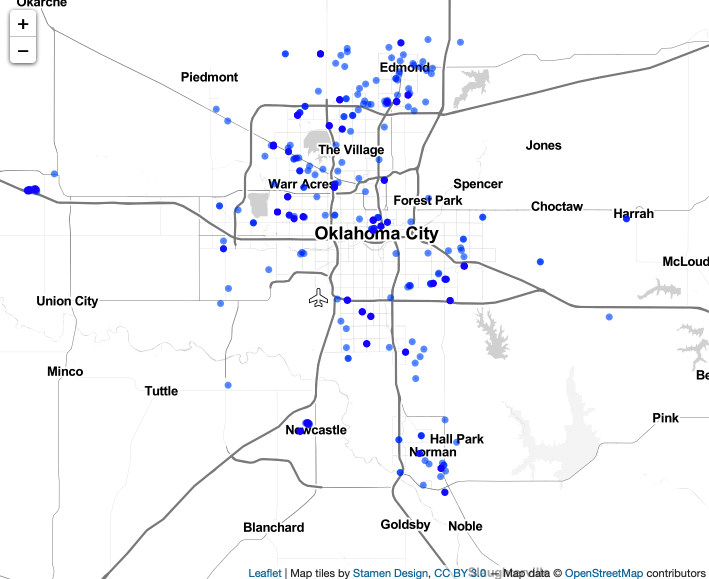
\includegraphics[height=3.5cm, width=4.5cm]{craigslist.mapfar.png}
           \caption{OKC Craigslist listings from April 26, 2021}
           \end{tabular}
           & \begin{tabular}{l}
             \parbox{0.5\linewidth}{%  change the parbox width as appropiate
             \textbf{Craigslist is an important data source for rental markets all over the country.}  
     
      Each Craigslist listing is required to include:       
        \begin{itemize}
            \item advertised rent price
            \item user-generated description of the unit
            \item Optional: square footage, number of bedrooms/bathrooms, and other  descriptions about amenities 
        \end{itemize}
    }
         \end{tabular}  \\
         \end{tabular}
\end{frame}

\begin{frame}[plain,c]
        \begin{center}
            \Large Does the extra information in Craigslist descriptions matter? What's the premium of extra information in the Craigslist rental market?
        \end{center}
\end{frame}

\begin{frame}[fragile]{Data Collection - Webscraping}
        \begin{itemize}
            \item Step 1: fill out baseurl ("https://oklahomacity.craigslist.org/search/apa")
            \item Step 2: build queries (bedrooms=2, bathrooms=1, sqft=900)
            \item Step 3: choose which attributes to extract from each listing (ID, title, price, sqft, etc...)
            \item Step 4: coerce code into a for loop to iterate through all listings within the query
            \item Step 5: organize and clean data
        \end{itemize}
\end{frame}

\begin{frame}[fragile]{Methods}
    \begin{equation}
    Y_{logrent}=\left(\begin{tabular} {l}
    \beta_{0} + \beta_{1}X_{sqft} + \beta_{2} X_{bdrms} + \beta_{3}X_{p.QDAP} + \beta_{4}X_{wordcount} \\ + \beta_{5}X_{t.wordcount}+\beta_{6}X_{t.direction} + \varepsilon,
    \end{tabular}\right)
    \end{equation}
    \begin{itemize}
        \item where $Y_{logrent}$ is log transformation of a continuous variable describing the price of each rental listing
        \item $X_{sqft}$ is the square footage of the rental unit, $X_{bdrms}$ is the number of bedrooms, $X_{p.QDAP}$ is the positivity index from the listing's description, $X_{wordcount}$ and $X_{t.wordcount}$ are the word counts for the description and the title, respectively, and $X_{t.direction}$ describes the sentiment of the listing title (positive, neutral, negative).
    \end{itemize}
\end{frame}

\begin{frame}{Research Findings}

\begin{table}[ht]
\caption{OLS estimates}
\centering
\begin{threeparttable}
\begin{tabular}{lccc}
\toprule
                            & Estimate    & Std. Error & P-value \\
\midrule
sqft        & 7.038e-04***   & (2.987e-05)    & $<2e-16$    \\
bdrms  & -1.951e-01***   & (11.623e-02)   & $<2e-16$ \\
p.QDAP        &      3.150e-01 & (1.657e-01)  & 0.0576 \\
wordcount     &    1.705e-03***  & (9.364e-05)    & $<2e-16$\\
t.wordcount & -8.005e-02*  & (3.837e-03) & 0.0372 \\
t.directionneutral & 6.785e-02 & (3.772e-02) & 0.0723 \\
t.directionpositive & 8.630e-02* & (3.731e-02) & 0.0209 \\
\bottomrule
\end{tabular}
\footnotesize Notes: Standard errors in parentheses. ***Significantly different from zero at the .1\% level; **Significantly different from zero at the 1\% level. *Significantly different from zero at the 5\% level. 
\end{threeparttable}
\end{table}

\end{frame}
\begin{frame}{Interpreting the Coefficients}

\begin{table}[ht]
\caption{Interpreting $\hat{\beta_i}$ Values}
\centering
\begin{threeparttable}
\begin{tabular}{lc}
\toprule
                            & \% Change in Rent\\
\midrule
sqft        & .07\%  \\
bdrms  & -17.72\% \\
p.QDAP        &  37\% \\
wordcount     &    0.171\% \\
t.wordcount & -0.797\% \\
t.directionneutral & 7.02\% \\
t.directionpositive & 9.01\% \\
\bottomrule
\end{tabular}
\footnotesize Notes: This value is found by exponentiating the $\hat{\beta_i}$ estimate, subtracting 1, and multiplying by 100 to find the \% in Y from a one-unit change in $X_i$. Equation: $ exp($\hat{\beta_i}$) - 1 * 100$.
\end{threeparttable}
\end{table}
    
\end{frame}


\begin{frame}{What did we learn? Why was it important? }
    \begin{itemize}
        \item For every additional word in a unit description, the rental price rises by about 0.2\%
        \item For every additional word in a unit title, the rental price falls by about 0.8\%
        \item Positive titles have a higher premium than neutral titles (all else equal) 
        \item Units with higher rent prices often have detailed unit descriptions and snappy, positive listing titles
        \item The relationship between the positivity of a listing's description and the rental price is large in magnitude even if it's not statistically significant (37\% increase for a one-unit change in the positivity index)
       \end{itemize}
\end{frame}

\begin{frame}{What did we learn? Why was it important? }
In Oklahoma City, like in many cities across the United States, there exists a rental market that Craigslist is uniquely able to summarize. Traditional data sources that cover rental markets in the United States are not able to release data at a fast enough pace to accurately characterize the market as it changes. With an introductory knowledge of webscraping, it is relatively painless to analyze data from a local Craigslist subdomain in real time. 
\end{frame}

\end{document}
